\graphicspath{{images/act_1.4/}}
\subsection{Cartesian space PD control}
\label{subsec:cartesian_space_PD_control}
The objective of this activity is to control movement of the ur5 robot end-effector so that it follows the Cartesian sinusoidal reference trajectory of activity \ref{subsec:generate_sinusoidal_reference}. The simulation starts with initial joint configuration $\mathbf{q_0}=\begin{bmatrix} 0.0 & -1.0 & 1.0 & 0.5 & 0.0 & 0.5 \end{bmatrix}$ rad and end-effector $\mathbf{p_0}=\begin{bmatrix}  0.577 &   0.192 &   0.364 \end{bmatrix}$~m. Likewise, the Cartesian sinusoidal reference trajectory starts at $\mathbf{p_0}$. Finally, movement of the ur5 robot is controlled with a proportional-derivative control method at Cartesian level. Thus, control law can be computed as 
\begin{equation}
	\boldsymbol{\tau}
	= \mathbf{J^T} (\mathbf{K_p e} + \mathbf{K_d \dot{e}}),
	\label{eq:cartesian_PD_control}
\end{equation}
\noindent where $\mathbf{J}$ is jacobian matrix, $\mathbf{e}=\mathbf{p_{des} - p}$ is end-effector position error, and $\mathbf{K_p, K_d}$ are the proportional and derivative gains respectively. \vspace{.5cm}

The Algorithm \ref{lst:cartesian_PD_control} control the movements of ur5 robot end-effector to track the Cartesian sinusoidal reference trajectory of activity~\ref{subsec:generate_sinusoidal_reference}. In this file, the PD control method is configured with ${K_{p}}=1000$ $\mathrm{\frac{N}{m}}$ and $K_{d}= 300$ $\mathrm{\frac{N.s}{m}}$. On one hand, Figure \ref{fig:act_1.4_ee_position} shows that trajectory tracking performance at the Cartesian space is poor because there are position, velocity and acceleration error. The constant position error in $z$-axis could be reduced by adding gravity terms on control law \eqref{eq:cartesian_PD_control}. On the other hand, Figure \ref{fig:act_1.4_joint_position} shows that angular trajectory of each joint with a PD at Cartesian space is different from angular trajectory obtained with a PD at joint space in activity \ref{subsec:inverse_kinematics_approach}. This is because the control law focuses on reducing the Cartesian position error of the end effector rather than position error of each joint. In this case, redundancy problem causes system to become unstable after $0.8$ seconds of simulation.  \vspace{.5cm}

\begin{lstlisting}[language=Python,caption=Move the ur5 robot end-effector so that it follows the Cartesian sinusoidal reference trajectory of activity \ref{subsec:generate_sinusoidal_reference}., label={lst:cartesian_PD_control}]
# =========================
#   Configuration of node
# =========================
# create a node: 
rospy.init_node("cartesian_PD_control")
# public in topic /joint_states	to send joint data	
pub = rospy.Publisher('joint_states', JointState, queue_size=1000)
# loop rate (in Hz)
rate 	= rospy.Rate(1000)		# 1000 [Hz]
dt 		= 1e-3					# 1  [ms]
# object(message) type JointState
jstate = JointState()

# ==========================================
#   Set initial joint configuration of UR5
# ==========================================
# initial configuration: position, velocity and acceleration 
q0 =   np.array([ 0.0, -1.0, 1.0, 0.5, 0.0, 0.5])
dq0 =  np.array([0.0, 0.0, 0.0, 0.0, 0.0, 0.0]) 
ddq0 = np.array([0.0, 0.0, 0.0, 0.0, 0.0, 0.0]) 

# desired trajectory: position, velocity and acceleration
q_des =   np.array([ 0.0, -1.0, 1.0, 0.5, 0.0, 0.5])
dq_des =  np.array([0.0, 0.0, 0.0, 0.0, 0.0, 0.0]) 
ddq_des = np.array([0.0, 0.0, 0.0, 0.0, 0.0, 0.0]) 

# measured trajectory: position, velocity and acceleration
q_med =   np.array([ 0.0, -1.0, 1.0, 0.5, 0.0, 0.5])
dq_med =  np.array([0.0, 0.0, 0.0, 0.0, 0.0, 0.0]) 
ddq_med = np.array([0.0, 0.0, 0.0, 0.0, 0.0, 0.0]) 

# ===========================
#   UR5 robot configuration
# ===========================
# joints name of UR5 robot
jnames = ['shoulder_pan_joint', 'shoulder_lift_joint', 'elbow_joint','wrist_1_joint', 'wrist_2_joint', 'wrist_3_joint']
# path of labs_ur5.urdf
urdf_path = os.path.join(pwd, "../../ur5_description/urdf/labs_ur5.urdf")
# the class robot load labs_ur5.urdf
ur5_robot = Robot(q0, dq0, dt, urdf_path)
# number of degress of freedom
ndof = ur5_robot.ndof

# create inertia matrix 
M = np.zeros([ndof,ndof])
# create nonlinear effects vector
b = np.zeros(ndof)
# create gravity vector
g = np.zeros(ndof)

# ==============================================
#   set initial cartesian configuration of UR5
# ==============================================
# initial cartesian configuration: position, velocity and acceleration
p0 = ur5_robot.get_ee_position()
dp0 = np.array([0.0, 0.0, 0.0])
ddp0 = np.array([0.0, 0.0, 0.0])

# desired cartesian trajectory: position, velocity and acceleration
p_des = copy(p0)
dp_des = np.array([0.0, 0.0, 0.0])
ddp_des = np.array([0.0, 0.0, 0.0])

# measured cartesian trajectory: position, velocity and acceleration
p_med = copy(p0)
dp_med = np.array([0.0, 0.0, 0.0])
ddp_med = np.array([0.0, 0.0, 0.0])

# ===============================
#   PD controller configuration
# ===============================
# proportional gain
kp = np.array([1000, 1000, 1000])   # N/m
# derivative gain   
kd = np.array([300, 300, 300])      # N.s/m
# control vector
tau = np.zeros(ndof)    

#===============
#   Simulation
#===============
t = 0.0             # [sec] 
sim_duration = 5.0  # [sec]
sine_duration = 4.0    # [sec]

while not rospy.is_shutdown():
    # desired cartesian trajectory
    p_des[0], dp_des[0], ddp_des[0] = sinusoidal_reference_generator(p0[0], 0.1, 1.5, sine_duration, t)

    # jacobian: position xyz [3x6]
    J = ur5_robot.jacobian(q_des)[0:3, 0:6]     
    
    # error: position and velocity
    e 	=  p_des - p_med
    de 	=  dp_des - dp_med    

    # PD control method (cartesian space)
    tau = J.T.dot( np.multiply(kp, e) + np.multiply(kd, de) )
    
    # send control signal
    ur5_robot.send_control_command(tau)
    # update states
    q_med, dq_med, ddq_med = ur5_robot.read_joint_position_velocity_acceleration()
    p_med, dp_med, ddp_med = ur5_robot.read_cartesian_position_velocity_acceleration()

    # publish message
    jstate.header.stamp = rospy.Time.now()
    jstate.name 		= jnames			# Joints position name
    jstate.position 	= q_med
    jstate.velocity 	= dq_med
    pub.publish(jstate)

    # update time
    t = t + dt
    
    # stop simulation
    if t>=0.8:
        print("stopping rviz ...")
        break
    rate.sleep()
\end{lstlisting}

\vspace*{0cm}
\begin{figure}[H]
	\centering
	\subfloat[]{
	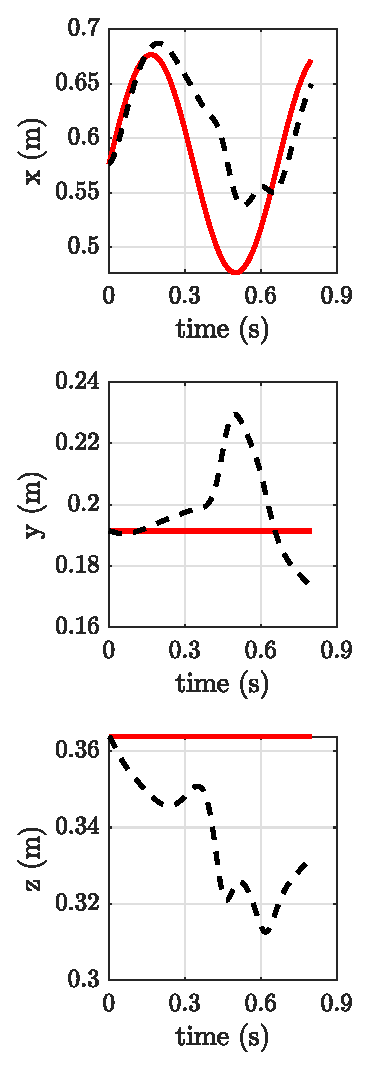
\includegraphics{ee_position.eps}
	}
	%\hfill
	\subfloat[]{
	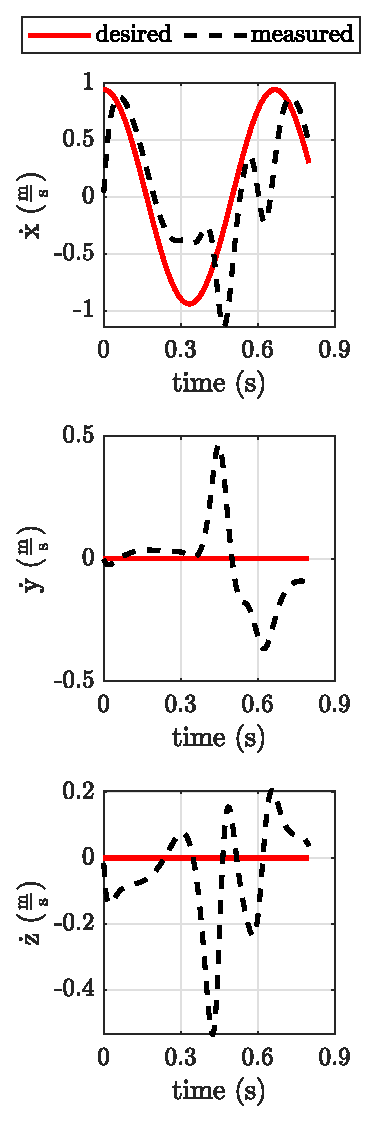
\includegraphics{ee_velocity.eps}
	}	
	%\hfill
	\subfloat[]{
	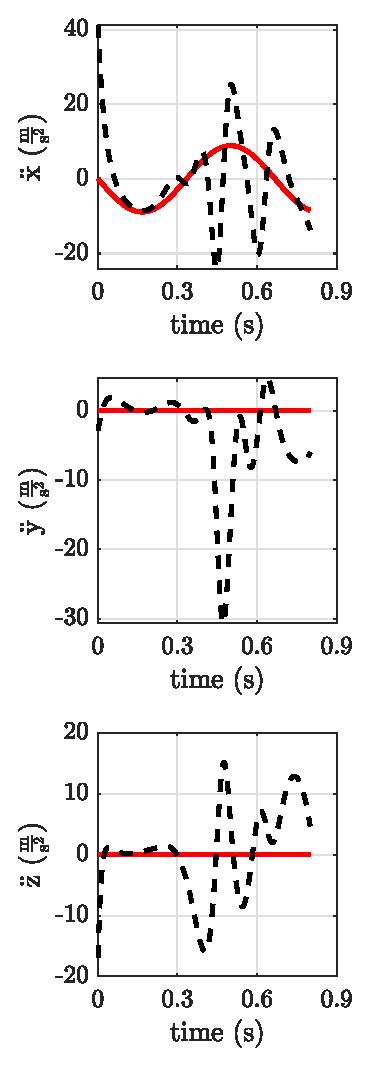
\includegraphics{ee_acceleration.eps}
	}		
	\caption{Trajectory tracking performances of the control method \eqref{eq:cartesian_PD_control} with  ${K_{p}}=1000$ $\mathrm{\frac{N}{m}}$ and $K_{d}= 300$ $\mathrm{\frac{N.s}{m}}$: (a) position, (b) velocity and (c) acceleration.}
	\label{fig:act_1.4_ee_position}
\end{figure}

\begin{figure}
    \centering
    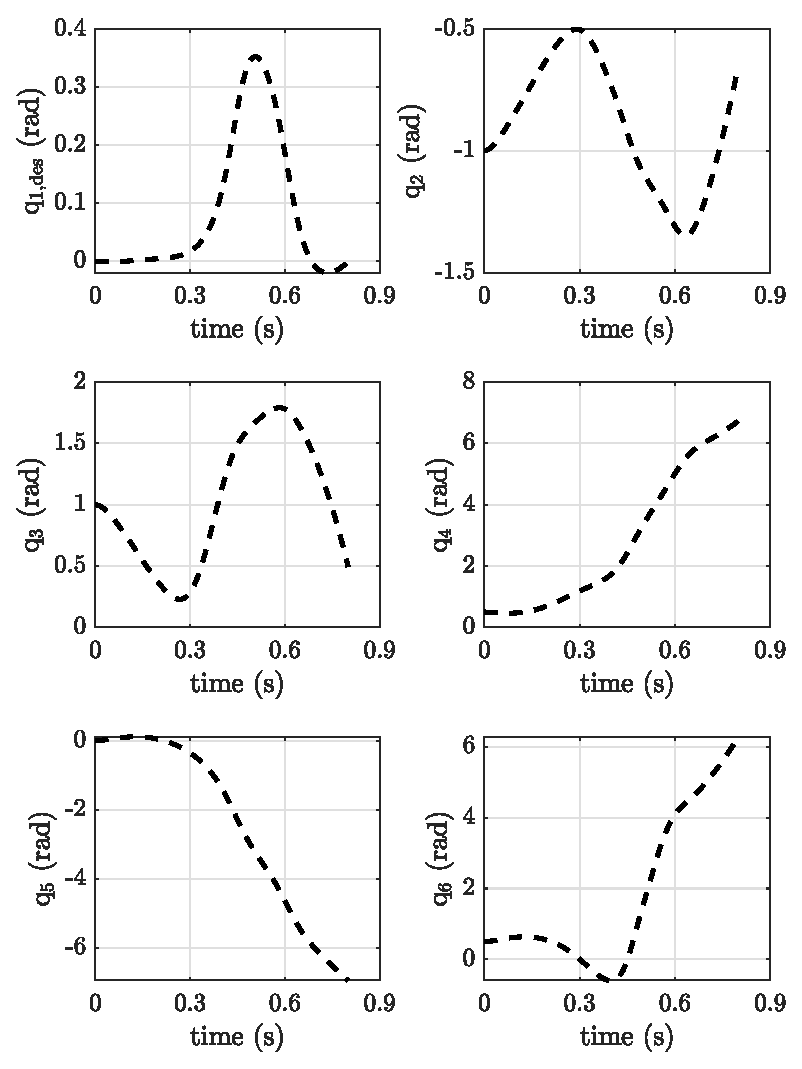
\includegraphics{joint_position.eps}	
    \caption{Angular position of each joint of UR5 robot with Algorithm \ref{lst:cartesian_PD_control}.}
    \label{fig:act_1.4_joint_position}
\end{figure}
